\documentclass[sigconf]{acmart}

\usepackage{setspace}
%\usepackage{enumerate}
\usepackage{enumitem}
\usepackage{booktabs} % For formal tables


% Copyright
%\setcopyright{none}
%\setcopyright{acmcopyright}
%\setcopyright{acmlicensed}
\setcopyright{rightsretained}
%\setcopyright{usgov}
%\setcopyright{usgovmixed}
%\setcopyright{cagov}
%\setcopyright{cagovmixed}


% DOI
\acmDOI{10.475/123_4}

% ISBN
\acmISBN{123-4567-24-567/08/06}

%Conference
\acmConference[TCSS 555: Spring 2018]{TCSS 555: Machine Learning Term Project}{June 2018}{Tacoma, WA USA} 
\acmYear{1997}
\copyrightyear{2016}

\acmPrice{15.00}


\begin{document}
\title{Mining Facebook Data via Text, Images, and Likes}
\titlenote{Produces the permission block, and
  copyright information}
\subtitle{Extended Abstract}
\subtitlenote{The full version of the author's guide is available as
  \texttt{acmart.pdf} document}


\author{Wenfei Yin}
\authornote{}
\orcid{}
\affiliation{%
  \institution{Institute of Technology}
  \streetaddress{Univ. of Washington: Tacoma}
  \city{Tacoma} 
  \state{WA} 
  \postcode{98402}
}
\email{yinwf@uw.edu}

\author{Shreya Yembarwar}
\authornote{}
\orcid{}
\affiliation{%
  \institution{Institute of Technology}
  \streetaddress{Univ. of Washington: Tacoma}
  \city{Tacoma} 
  \state{WA} 
  \postcode{98402}
}
\email{shreyay@uw.edu}

\author{Jonathan McFadden}
\authornote{}
\orcid{}
\affiliation{%
  \institution{Institute of Technology}
  \streetaddress{Univ. of Washington: Tacoma}
  \city{Tacoma} 
  \state{WA} 
  \postcode{98402}
}
\email{mcfaddja@uw.edu}



% The default list of authors is too long for headers}
\renewcommand{\shortauthors}{Wenfei Yin, Shreya Yembarwar, Jonathan McFadden}


\begin{abstract}
There is a growing interest in mining social media data for predictive applications in recommender systems, tailored advertisements, personalization in various domains etc. End applications include e-commerce, digital text forensics etc. Data from Facebook profiles was mined to predict the age group, gender, and personality information of unseen social media users.  The data consisted of profile pictures of the users, text (and a digest of that text) from users' posts, and 'likes' of a user.  For simplicity, the ages were grouped into four ranges.  Meanwhile, the personality information consisted of scores on a 5-part (score) personality
test/analysis.
\end{abstract}

%
% The code below should be generated by the tool at
% http://dl.acm.org/ccs.cfm
% Please copy and paste the code instead of the example below. 
%
\begin{CCSXML}
<ccs2012>
% <concept>
%  <concept_id>10003033.10003083.10003095</concept_id>
%  <concept_desc>Networks~Network reliability</concept_desc>
%  <concept_significance>100</concept_significance>
% </concept>
</ccs2012>  
\end{CCSXML}

%\ccsdesc[500]{Computer systems organization~Cloud based systems}
%\ccsdesc[300]{Computer systems organization~Software as a Service}
%\ccsdesc[300]{Computer systems organization~Containers Service}
%\ccsdesc[300]{Computer systems organization~Virtualization}
%\ccsdesc{Database systems~NoSQL}
%\ccsdesc{Virtualization methods~Containers}
%\ccsdesc[100]{Cloud Systems~Perfomance}
%\ccsdesc[100]{Cloud Systems~Cost}

% We no longer use \terms command
%\terms{Theory}

\keywords{ACM proceedings, \LaTeX, text tagging}


\maketitle

\section{Introduction}

mnbmb




%---------------------------------------------------
%---------------------------------------------------



\section{Methodology}

Since there were three different types of data, we have divided describing our methodology into three parts.  Each data type/source (\emph{text, images, \& likes}) will have its own part (\emph{section}).

\subsection{Text}

For the Text part, we separate it into three parts. The first one is using the text to predict the accuracy of age and gender, then we use the 82- LIWC features to predict the big five personalities. For each part, we also use different methods to build the basic model to test accuracy.

We tried four different methods in text part, Linear regression, Random forest, Na�ve Bayes and Logistical regression. Finally, we find the best result from the method which uses logistical regression and Na�ve regression.

The first step of the text part is data preprocessing. In the files, we find that they are separated, thus we merge the profile file and text file according to the common primary key in each take. We add each text part into profile.csv. At the meanwhile, we also transfer the age to age groups, and we use 1 and 0 to replace the female and male in order to more effective.

After data preprocessing, we use the Na�ve Bayes to predict the age and gender. As is known to us who focus on machine learning. Na�ve Bayes classifiers are a family of simple "probabilistic classifiers" based on applying Bayes theorem with strong independence assumptions between the features. However, we find the model only working well on gender part. The accuracy of age in Na�ve Bayes model is 0.49 which is lower than baseline (0.59). Therefore, we have to change our method. After researching, we guess the Logistical Regression will work well on age part. At the beginning, we split the training data into two part, the one is training data which are 8000 rows, the other is test data which is 1500 rows. To our surprise, it does not work well. After trying different methods, like linear regression, random forest. We find the model cannot work well when we use text to predict the age, thus we try to use 82-LIWC features to build model.

The LIWC, The linguistic Inquiry and Word Count tool, is known text analysis software which is widely used in psychology studies, In the file, for each user, it has 82 features. We have to merge the LIWC and profile file. When we create the model, we delete the big five personalities which need to be predicted in the table. After testing in local machine, we find it work well in age predict. The accuracy of age group reach to 0.62.

For Five Big Personality, we have to used 82-LIWC features. Because of big data, we decide to use Linear regression to set the model. In statistics, Linear regression is a linear approach to modeling the relationship between a scalar response and one or more explanatory variables. Fortunately, Linear regression work well in the model, the results almost similar with baseline. Although we try to decrease the RMSE of five big personality, the methods we tried are almost same. 


%---------------------------------------------------

\subsection{Images}

Convolutional Neural Networks was used to handle the image source of this experiment. CNN is a class of deep, feed forward ANN having applications in image/video processing, NLP etc. CNNs draw inspiration the animal vision cortex system. CNNs requires minimal preprocessing, i.e. the network learns the features as opposed to them being engineered. CNNs work by extracting features and recognizing patterns from the images, by convoluting the image with filters. 
CNNs have proved to be a robust and low error approach for the image classification tasks. The overlap between Machine Learning and Computer Vision has seen many recent technological developments, particularly Deep Learning. CNNs with deeper/wider layers and larger training datasets tend to perform better. 

In order to avoid over-fitting, data augmentation was performed on the image database. The augmentation operations included rescaling each pixel, flipping horizontally, rotating the image by variable degrees, randomly zooming into the image etc. 

A series of experiments was conducted, with different CNN models, before and after performing any filtering operations through Haar cascades. Only gender prediction was implemented with images, since experiments with age prediction did not give good results. 

%
\subsubsection{Image Model-1: Basic CNN Model}

Reference for this model was taken from the Keras blog\footnote{\textbf{Reference:} https://blog.keras.io/building-powerful-image-classification-models-using-very-little-data.html}.  The model had an input size of 224x224 pixels, with 3 convolutional layers and and one fully connected layer. The optimizer used was ?adam? and the the evaluation metric was ?accuracy?.  This model is described in \textbf{Table \ref{tab:img-model1}}.

\begin{table}
\caption{IMAGE MODEL-1: Basic CNN Model}
\label{tab:img-model1}
\begin{minipage}{\columnwidth}
	\begin{center}
	\begin{tabular}{l | c | c | c | c | c}
  	\toprule
		\textbf{Layer}		& \textbf{Filters}		& \textbf{Neurons}	& \textbf{Fltr. Sz}	& \textbf{Act.}	& \textbf{Dropout}	\\
		\hline
		Conv	\footnote{Convolutional}	& 32					& -					& $3 \times 3$		& relu			& -				\\
		Conv	\footnote{Convolutional}	& 32					& -					& $3 \times 3$		& relu			& -				\\
		Conv	\footnote{Convolutional}	& 64					& -					& $3 \times 3$		& relu			& -				\\
		Full-Con\footnote{Fully Connected}	& -					& 64					& -				& relu			& 0.5				\\
		Output			& -					& 1					& -				& sigmoid			& -				\\
	\bottomrule
	\end{tabular}
	\end{center}
\bigskip
\footnotesize
  \emph{Note:} Fltr. Sz = Filter Size \\
  \emph{Note:} Act. = Activation Function
\end{minipage}
\end{table}

%
\subsubsection{Image Model-2: RESNET50}

Bottleneck features were extracted from the RESNET50 model. Final layer of the model was not included. The pre-trained weights were used to find the bottleneck values, i.e. features were extracted. Fully connected layers were added to run with the training data. This model is described in \textbf{Table \ref{ }}.


%---------------------------------------------------

\subsection{Likes}

When considering the Likes data, we first create a \textbf{User/LikeID Matrix} from the training data we are given.  This process is described below in the Dataset and Metrics section. Based on the training data we were given, this resulted in a matrix with 536204 columns.  Due to the large number of columns in this matrix, dimensionality reduction using Singular Value Decomposition or Principal Components Analysis was considered.  Unfortunately, when the singular values of this matrix were computed (\emph{up to the 9499th singular value}), there was no characteristic "cliff" drop-off in their magnitudes which would indicate a good point for truncation.  

To illustrate this, the type of "cliff" in the singular value magnitudes we were seeking can be seen in the plot of singular value magnitudes, from a different dataset given in \textbf{Figure 1}.

\begin{figure}
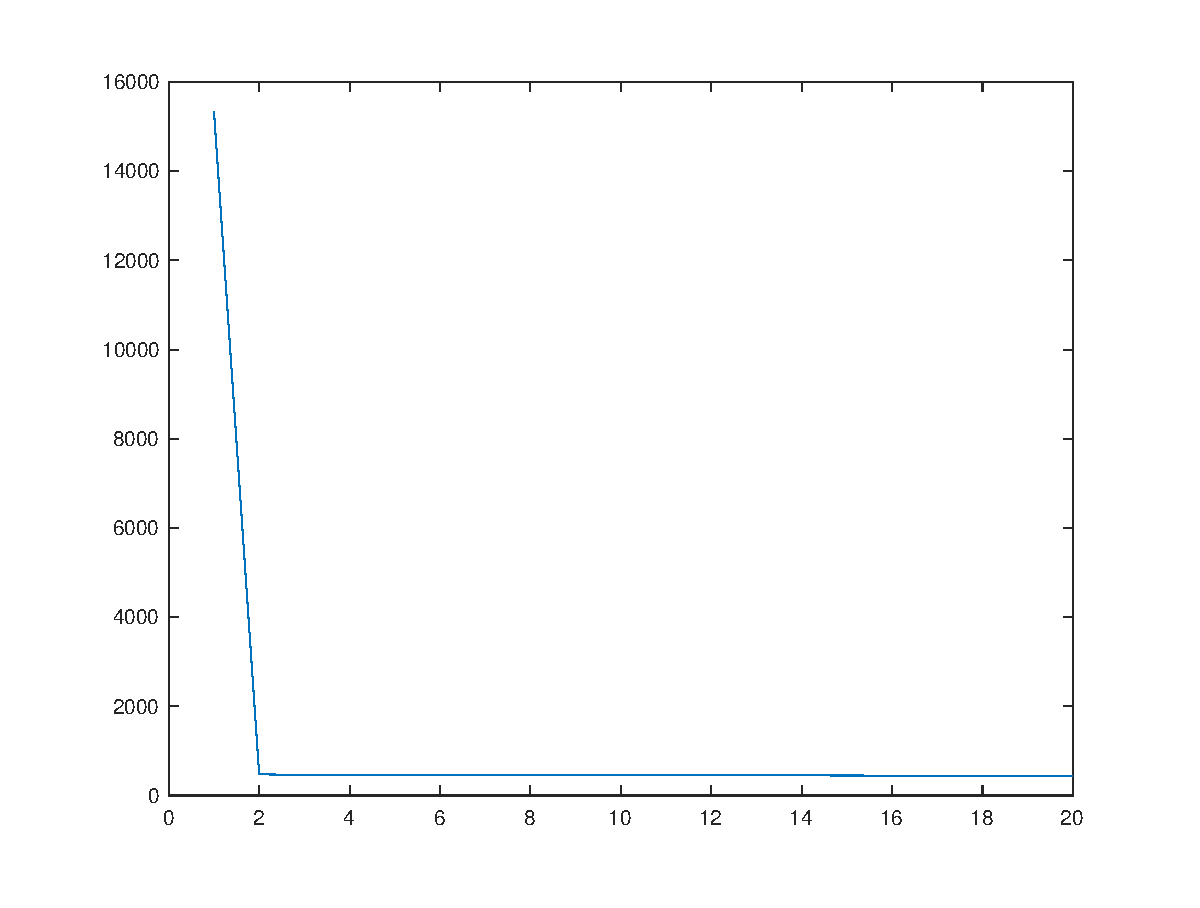
\includegraphics[width=3.5in]{cliffWANTEDa}
\caption{The type of 'cliff' drop-off in singular value magnitudes we wanted to see.}
\end{figure}

Unfortunately, the result was got did not have the sudden drop over just a few singular values.  What we got instead can be seen in \textbf{Figure 2}.

\begin{figure}
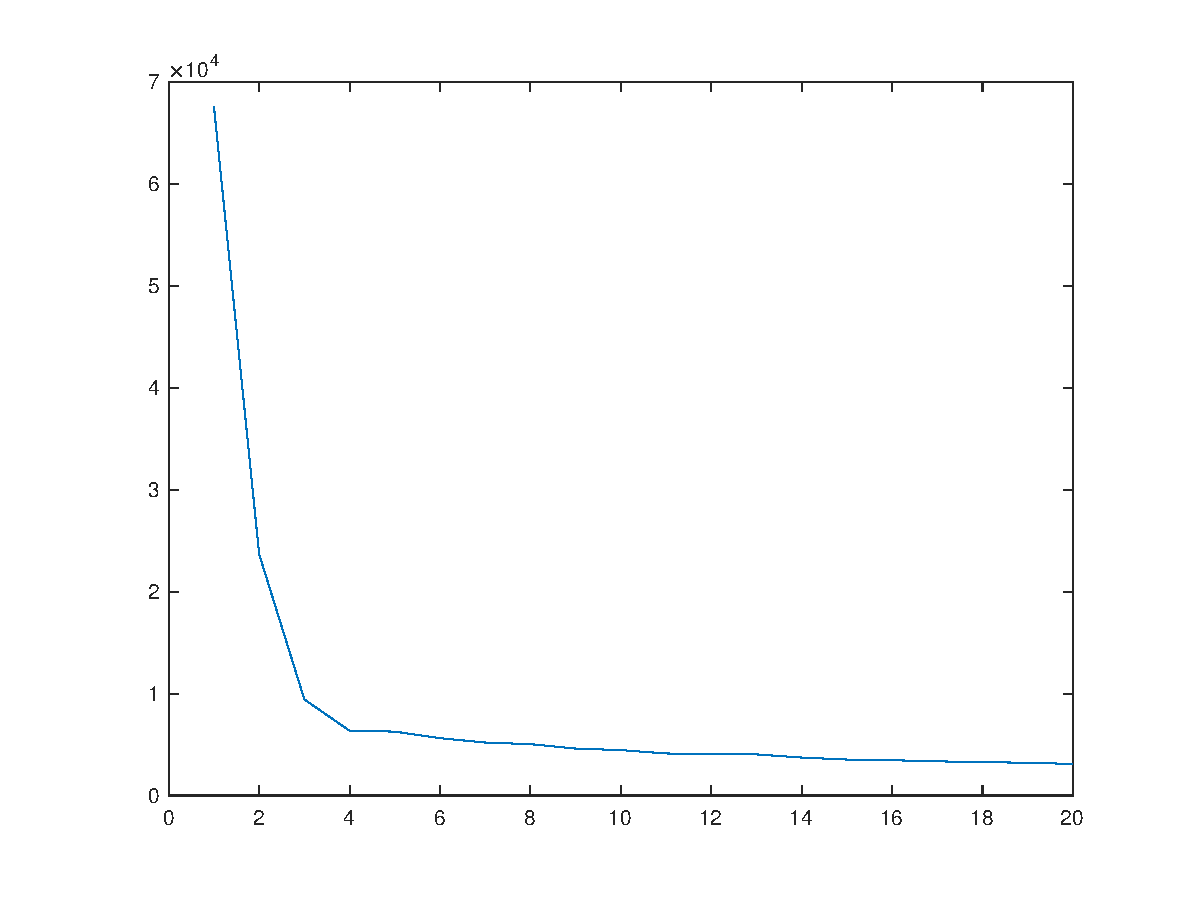
\includegraphics[width=3.5in]{cliffGOT}
\caption{The singular value magnitudes we got instead of what we wanted to see.}
\end{figure}

Thus, we proceeded to use the entirety of the column space of the \textbf{User/LikeID Matrix}.  We constructed models using the machine learning algorithms

\begin{itemize}
	\item	Random Forest
	\item AdaBoost
	\item Bagging (\emph{with in-bag scoring})
	\item Bagging (\emph{with out-of-bag scoring})
	\item Naive Bayes
	\item	K-Nearest Neighbor
	\item	Support Vector Machine
	\item Linear Support Vector Machine
	\item Gradient Boosting
	\item Neural Networks (\emph{implemented using Keras})
\end{itemize}

Each of these algorithms was run using a variety of performance parameters, including the number of estimators, the learning rate, the tolerance, the number of neighbors, and more.  Ultimately, for each of the user attributes, we chose the algorithms and settings

\begin{itemize}
	\item \textbf{\underline{Age Group}: Neural Network} with \textbf{750 base nodes} (\emph{see below for full network design} \\
	\item \textbf{\underline{Gender}: Neural Network} with \textbf{650 base nodes} (\emph{see below for full network design} \\
	\item \textbf{\underline{OPE}: SVM} with \textbf{tolerance of $1 \times 10^{-6}$} \\
	\item	 \textbf{\underline{NEU}: AdaBoost} with \textbf{100 estimators and a learning rate of 1.0} \\
	\item	 \textbf{\underline{EXT}: Random Forest} with \textbf{1500 estimators} \\
	\item	 \textbf{\underline{AGR}: Bagging \emph{using in-bag scoring}} with \textbf{250 estimators} \\
	\item	 \textbf{\underline{CON}: Bagging \emph{using in-bag scoring}} with \textbf{100 estimators}
\end{itemize}

We also strongly considered the alternative algorithms and settings

\begin{itemize}
	\item	 \textbf{\underline{NEU}: AdaBoost} with \textbf{250 estimators and a learning rate of 0.01} \\
	\item	 \textbf{\underline{EXT}: K-Nearest Neighbors} with \textbf{500 neighbors} \\
	\item	 \textbf{\underline{AGR}: K-Nearest Neighbors} with \textbf{800 neighbors} \\
	\item	\textbf{\underline{CON}: AdaBoost} with \textbf{1000 estimators and a learning rate of 1.0}
\end{itemize}

%
\subsubsection{Neural Net Design}

We designed three types of neural networks for this part of the project.  The first type of neural net was a single-class binary classifier for predicting gender; while second type as a multi-class binary classifier for predicting age group.  Finally, the last type of neural net we designed was a multilayer linear regressor.  All three networks had the same number of hidden and dropout layers, however they used different activation functions and kernel initializers.  Additionally, all of these neural networks were implemented in \textbf{Keras} using its \textbf{Sequential} model.  We summarize the three neural nets in \textbf{Table \ref{tab:like-nnets}}.

\begin{table}
\caption{Likes SUMMARY of Neural Nets}
\label{tab:like-nnets}
\begin{minipage}{\columnwidth}
	\begin{center}
	\begin{tabular}{l | c | c | c }
  	\toprule
						& \textbf{Gender}	& \textbf{Age Group}		& \textbf{Regressor}	\\
		\hline
		\hline
		Input Layer		&				&					&				\\
		$\qquad$ Neurons	& 536204			& 536204				& 536204			\\
		\hline
		1st Hidden Layer	&				&					&				\\
		$\qquad$ Dense	& 975			& 1125				& 750			\\
		$\qquad$ Kernel	& \emph{uniform}	& \emph{default}		& \emph{default}	\\
		$\qquad$ Activation	& \emph{relu}		& \emph{relu}			& \emph{relu}		\\
		\hline
		1st Dropout Layer	& 0.25			& 0.25				& 0.25			\\
		\hline
		2nd Hidden Layer	&				&					&				\\
		$\qquad$ Dense	& 1300			& 1500				& 1000			\\
		$\qquad$ Kernel	& \emph{uniform}	& \emph{default}		& \emph{default}	\\
		$\qquad$ Activation	& \emph{relu}		& \emph{softmax}		& \emph{relu}		\\
		\hline
		2nd Dropout Layer	& 0.375			& 0.375				& 0.375			\\
		\hline
		3rd Hidden Layer	&				&					&				\\
		$\qquad$ Dense	& 975			& 1125				& 750			\\
		$\qquad$ Kernel	& \emph{uniform}	& \emph{default}		& \emph{default}	\\
		$\qquad$ Activation	& \emph{sigmoid}	& \emph{sigmoid}		& \emph{sigmoid}	\\
		\hline
		3rd Dropout Layer	& 0.25			& 0.25				& 0.25			\\
		\hline
		4th Hidden Layer	&				&					&				\\
		$\qquad$ Dense	& 650			& 750				& 500			\\
		$\qquad$ Kernel	& \emph{uniform}	& \emph{default}		& \emph{default}	\\
		$\qquad$ Activation	& \emph{relu}		& \emph{relu}			& \emph{sigmoid}	\\
		\hline
		Output Layer		&				&					&				\\
		$\qquad$ Neurons	& 1				& 4					& 1				\\
		$\qquad$ Kernel	& \emph{uniform}	& \emph{default}		& \emph{default}	\\
		$\qquad$ Activation	& \emph{sigmoid}	& \emph{softmax}		& \emph{sigmoid}	\\
	\bottomrule
	\end{tabular}
	\end{center}
\bigskip
\end{minipage}	
\end{table}



%---------------------------------------------------
%---------------------------------------------------



\section{Dataset and Metrics}

dadfsfa


\subsection{Text}

There are five filed in the training dataset. LIWC, profile, relation and test. For text and LIWC part, we use the text folder which contain 9500 text files, and we merge text files and a csv file named "profile.csv" because of common primary key "userid". Meanwhile, we merge the profile and the LIWC file as well. In the profile, we use 0 denote male, and 1 is female. In the age, we have classified the age likes "xx-24", "25-34", "35-69", and "50-xx". In order to more effective, the big five personality, Openness, Conscientiousness, Extroversion, Agreeableness, Emotional Stability, being referred to as "ope", "con", "ext", "agr" and "neu".


%---------------------------------------------------

\subsection{Likes}

dfasdfasdf


%---------------------------------------------------

\subsection{Images}

The image database contained 9500 images, which was split into 8000 for training and 1500 for validation. For the purposes of gender prediction, the 8000 images were regrouped according to the labels, i.e. 3386 males and 4614 females. The regrouping was done using the profile.csv file. One critical issue to note is that it is an unbalanced distribution between the two labels. 
Some of the issues noticed in the database were as follows:

\begin{itemize}
	\item	Images did not contain faces
	\item	Images contained multiple faces
	\item Images did not contain face belonging to the label holder
\end{itemize}

The third issue mentioned above cannot be tackled, as the system lacks that intelligent ability. Operations can be implemented to filter the images with the first two issues mentioned above. OpenCV Haar Cascades were used as the filters. Haar cascades is a method used for object detection in images. There are specialized .xml files present, for detection of various objects. These files are created by a machine learning approach where a cascade function is trained from a lot of positive and negative images. 
The cascade functions customized for face detection were used in this project, to filter images which had multiple faces or images which did not contain faces. The cascade functions used were for different views of a face, i.e. frontal and profile views. The images which passed through at least one cascade were retained. Manual selection was performed on the few residual images, to perform a final filtering operation. 

%
\subsubsection{Image Metrics}

This project contains usage of various machine learning algorithms, which are either classification or regression. The evaluation metric of ?accuracy? was used for the classification models, and ?root mean squared error? for the regression models. 




%---------------------------------------------------
%---------------------------------------------------


\section{Results}

Our overall results can be summarized by the table .

% table here

Detailed results for the three different classes of data are given in their own sections below.


%---------------------------------------------------

\subsection{Text}

For age prediction model, using Logistical regression based on 82-LIWC features is best choice in the method we tried. We also use other methods, line Linear regression, random forest, Na�ve Bayes. We can see the results in the chart given in \textbf{Table \ref{tab:txt-ageSEX}}.

\begin{table}
\caption{Text RESULTS for Age \& Gender Accuracy}
\label{tab:txt-ageSEX}
\begin{minipage}{\columnwidth}
	\begin{center}
	\begin{tabular}{l | c | c}
  	\toprule
							& \textbf{Age Group}				& \textbf{Gender}	\\
		\hline
		\hline
   		Baseline				& 0.59						& 0.59			\\
		\hline
		Linear Regression		& 0.52						& 0.60			\\
		\hline
		Random Forest			& 0.51						& 0.60			\\
		\hline
		Naive Bayes			& 0.49						& 0.71			\\
		\hline
		Logistical Regression	& 0.61\footnote{Using LIWC data}	& 0.59			\\
							& 0.59\footnote{Using text data}	& 				\\
	\bottomrule
	\end{tabular}
	\end{center}
\bigskip
\end{minipage}	
\end{table}

From the chart in \textbf{Table \ref{tab:txt-ageSEX}}, we can see that the best result in age prediction is the model when it uses logistical regression based on LIWC, and the best accuracy in gender predict model is Na�ve Bayes. Therefore, our choice are Na�ve Bayes based on text in gender and Logistical Regression based on LIWC in age prediction.

For Big five personality, we only use linear regression on the text and LIWC part, because we tried other methods, and the results are same. The results are in the chart given in \textbf{Table \ref{tab:txt-person}}.

\begin{table}
\caption{Text RESULTS for Personality Score RMSE}
\label{tab:txt-person}
\begin{minipage}{\columnwidth}
	\begin{center}
	\begin{tabular}{l | c | c | c | c | c}
  	\toprule
						& \textbf{OPE}	& \textbf{NEU}	& \textbf{EXT}	& \textbf{AGR}	& \textbf{CON}	\\
		\hline
		Baseline			& 0.65		& 0.80		& 0.79		& 0.66		& 0.73		\\
		Linear Regression	& 0.65		& 0.79		& 0.79		& 0.65		& 0.72		\\
	\bottomrule
	\end{tabular}
	\end{center}
\bigskip
\end{minipage}
\end{table}

From the chart in \textbf{Table ref{tab:txt-person}}, we can clearly see that the results under the predict model are similar with Baseline when we use Linear regression.


%---------------------------------------------------

\subsection{Images}

jhlgjhg


%---------------------------------------------------

\subsection{Likes}

ljlkj



%---------------------------------------------------
%---------------------------------------------------


\section{Conclusion}

ljhgljhg


\subsection{Text}

For text part, we have tried many methods when we set up the model, but we do not have do more specific work on data preprocessing, such as feature selection, word choice. When we predict the age and gender, we can find more significant words, like she, he which will affect our results. Although we get a good result in the age prediction when we use Logistical regression based on 82 LIWC features, it is not perfect. In our last assignment, we find the neural network may be good at decrease RMSE in big five personality, thus we can try it in the future work. 


%---------------------------------------------------

\subsection{Images}

jbklj


%---------------------------------------------------

\subsection{Likes}

bljk









































































\bibliographystyle{ACM-Reference-Format}
\bibliography{sigproc} 

\end{document}
